\chapter{Теоретические вопросы}

\section{Сформулировать определения случайной величины и функции распределения вероятностей случайной величины. Записать основные свойства функции распределения}

Пусть $(\Omega, \mathcal{B}, P)$ - вероятностное пространство. \textbf{Случайной величиной} $X$ будем называть отображение: $X : \Omega \rightarrow \mathbb{R}$.

\textbf{Функцией распределения вероятностей случайной величины} $X$ называется отображение: $F_X : \mathbb{R} \rightarrow \mathbb{R}$, определенное правилом: $F_X(x) = P\{X < x\}$.

\textbf{Свойства}:
\begin{enumerate}
	\item $\forall x \in \mathbb{R} : 0 \leq F(x) \leq 1$;
	\item если $x_1 \leq x_2$, то $F(x_1) \leq F(x_2)$, т.е. $F$ является неубывающей функцией;
	\item $\lim_{x \to -\infty} F(x) = 0$, $\lim_{x \to +\infty} F(x) = 1$;
	\item $P\{x_1 \leq X < x_2\} = F(x_2) - F(x_1)$;
	\item $\lim_{x \to x_0-} F(x) = F(x_0)$, т.е. $F$ непрерывна слева в каждой точке.
\end{enumerate}

\section{Сформулировать определение дискретной случайной величины; понятие ряда распределения. Сформулировать определение непрерывной случайной величины и функции плотности распределения вероятностей}

Случайная величина называется \textbf{дискретной}, если она принимает конечное или счетное множество значений.

Закон распределения дискретной случайной величины принимающей конечное множество значений можно задать с помощью таблицы вида:

\begin{tabular}{|>{\columncolor[gray]{0.8}}c|c|c|c|c|}
	\hline
	X & $x_1$ & $x_2$ & ... & $x_n$ \\ \hline
	$P$ & $p_1$ & $p_2$ & $...$ & $p_n$ \\ \hline
\end{tabular}

Здесь $p_i = P\{X=x_i\}, i = \overline{1, n}$. Такая таблица называется \textbf{рядом распределения} дискретной случайной величины $X$.

Случайная величина $X$ называется \textbf{непрерывной}, если существует функция: $f: \mathbb{R} \rightarrow \mathbb{R}$ такая, что функцию случайной величины $X$ можно представить в виде: $\forall x \in \mathbb{R}: F(x) = \int_{-\infty}^{x} f_X(t) \, dt$. При этом $f$ называется \textbf{функцией плотности распределения вероятностей} случайной величины $X$.

\section{Сформулировать определение непрерывной случайной величины. Записать основные свойства функции плотности распределения вероятностей непрерывной случайной величины}

Случайная величина $X$ называется \textbf{непрерывной}, если существует функция: $f: \mathbb{R} \rightarrow \mathbb{R}$ такая, что функцию случайной величины $X$ можно представить в виде: $\forall x \in \mathbb{R}: F(x) = \int_{-\infty}^{x} f_X(t) \, dt$.

\textbf{Свойства}:
\begin{enumerate}
	\item $f(x) \geq 0, x \in \mathbb{R}$;
	\item $P\{x_1 \leq X < x_2\} = \int_{x_1}^{x_2} f(x) \, dx$;
	\item $\int_{-\infty}^{+]infty} f(x) \, dx = 1$ (условие нормировки);
	\item Если $\Delta x$ мало, а $x_0$ - точка непрерывности функции $f$, то $P\{x_0 \leq X < x_0 + \delta x\} \approx f(x_0)\Delta x$;
	\item Если $X$ - непрерывная случайная величина, то для любого, наперед заданного $x_0: P\{X=x_0\} = 0$.
\end{enumerate}

\section{Сформулировать определения случайного вектора и его функции распределения вероятностей. Записать свойства функции распределения двумерного случайного вектора}

Пусть:
\begin{enumerate}
	\item $(\Omega, \mathcal{B}, P)$ - вероятностное пространство;
	\item случайные величины $X_1(w), ..., X_n(w)$ заданы на этом вероятностном пространстве.
\end{enumerate}

n-мерным \textbf{случайным вектором} (n-мерной случайной величиной) называется кортеж $\vec{X} = (X_1(w), ..., X_n(w))$. При этом, случайная величина $X_i(w)$ называется i-ой координатой вектора $\vec{X}$.

\textbf{Свойства} (n=2):
\begin{enumerate}
	\item $0 \leq F(x_1, x_2) \leq 1$;
	\item а) при фиксированном $x_2$ функция $F(x_1, x_2$) как функция переменной $x_1$ является неубывающей. б) ---//--- $x_1$ ---//--- $x_2$ ---//---;
	\item $\lim_{x_1 \to -\infty} F(x_1, x_2) = \lim_{x_2 \to -\infty} F(x_1, x_2) = 0$;
	\item $\lim_{x_1 \to +\infty, x_2 \to +\infty} F(x_1, x_2) = 1$;
	\item $\lim_{x_1 \to +\infty, x_2 = const} F(x_1, x_2) = F_{X_2}(x_2)$, $\lim_{x_1 = const, x_1 \to +\infty} F(x_1, x_2) = F_{X_1}(x_1)$;
	\item $P\{a_1 \leq X_1 < b_1, a_2 \leq X_2 < b_2\} = F(a_1, a_2) + F(b_1, b_2) - F(a_1, b_2) - F(b_1, a_2)$;
	\item а) при фиксированном $x_2$ функция $F(x_1, x_2$) как функция переменной $x_1$ является непрерывной во всех точках. б) ---//--- $x_1$ ---//--- $x_2$ ---//---.
\end{enumerate}

\section{Сформулировать определение дискретного случайного вектора; понятие таблицы распределения двумерного случайного вектора. Сформулировать определения непрерывного случайного вектора и его функции плотности распределения вероятностей}

\textbf{Случайный вектор} $\vec{X} = (X_1, ..., X_n)$ называется \textbf{дискретным}, если каждая из случайных величин $X_i = \overline{1, n}$ является дискретной.

Пусть:
\begin{enumerate}
	\item $(X, Y)$ -- двумерный случайный дискретный вектор;
	\item будем считать, что $X$ и $Y$ принимают конечное множество значений: $X \in \{x_1, ..., x_m\}, Y \in \{y_1, ..., y_n\}$. Это означает, что случайный вектор $(X, Y)$ может принимать значения $(x_i, y_i), i = \overline{1, m}, j = \overline{1, n}$.
\end{enumerate}

Закон распределения такого вида задают с использованием таблицы:

\begin{tabular}{|c|c|c|c|c|c|c|}
	\hline
	  & $y_1$ & ... & $y_j$ & ... & $y_n$ & $P_X$ \\ \hline
	$x_1$ & $p_{11}$ & ... & $p_{1j}$ & ... & $p_{1n}$ & $P_{X1}$ \\ \hline
	... & ... & ... & ... & ... & ... & ... \\ \hline
	$x_i$ & $p_{i1}$ & ... & $p_{ij}$ & ... & $p_{in}$ & $P_{Xi}$ \\ \hline
	... & ... & ... & ... & ... & ... & ... \\ \hline
	$x_m$ & $p_{m1}$ & ... & $p_{mj}$ & ... & $p_{mn}$ & $P_{Xm}$ \\ \hline
	$P_Y$ & $P_{Y1}$ & ... & $P_{Yj}$ & ... & $P_{Yn}$ & 1 \\ \hline
\end{tabular}

Случайный вектор $\vec{X} = (X_1, ..., X_n)$ называется \textbf{непрерывным}, если существует функция $f(x_1, ..., x_n): F(x_1, ..., x_n) = \int_{-\infty}^{x_1} \, dt_1 \cdot ... \cdot \int_{-\infty}^{x_n} f(t_1, ..., t_n) \, dt_n$, где $F$ -- функция распределения вектора $(X_1, ..., X_n)$.

Функция $f(x_1, ..., x_n) = \frac {\delta^n F(x_1, ..., x_n)}{\delta x_1 \cdot ... \cdot \delta x_n}$ называется (совместной) \textbf{плотностью распределения вероятностей}.

\section{Сформулировать определения непрерывного случайного вектора и его функции плотности распределения вероятностей. Записать основные свойства функции плотности распределения двумерных случайных векторов}

Случайный вектор $\vec{X} = (X_1, ..., X_n)$ называется \textbf{непрерывным}, если существует функция $f(x_1, ..., x_n): F(x_1, ..., x_n) = \int_{-\infty}^{x_1} \, dt_1 \cdot ... \cdot \int_{-\infty}^{x_n} f(t_1, ..., t_n) \, dt_n$, где $F$ -- функция распределения вектора $(X_1, ..., X_n)$.

Функция $f(x_1, ..., x_n) = \frac {\delta^n F(x_1, ..., x_n)}{\delta x_1 \cdot ... \cdot \delta x_n}$ называется (совместной) \textbf{плотностью распределения вероятностей}.

\textbf{Свойства} (n=2):
\begin{enumerate}
	\item $f(x_1, x_2) \geq 0$;
	\item $P\{a_1 \leq X_1 < b_1, a_2 \leq X_2 < b_2\} = \int_{a_1}^{b_1} \, dx_1 \cdot \int_{a_2}^{b_2} f(x_1, x_2)\, dx_2$;
	\item $\int \int_{\mathbb{R}} f(x_1, x_2)\, dx_1dx_2 = 1$;
	\item $P\{x_1 \leq X_1 < x_1 + \Delta x_1, x_2 \leq X_2 < x_2 + \Delta x_2\} \approx f(x_1, x_2) \cdot \Delta x_1 \cdot \Delta x_2$, если $(x_1, x_2)$ -- точки непрерывности;
	\item Для любого, наперед заданного $(x_1^\circ, x_2^\circ): P\{(X_1, X_2) = (x_1^\circ, x_2^\circ)\} = 0$, если $(X_1, X_2)$ -- непрерывный случайный вектор;
	\item $P\{(X_1, X_2) \in D\} = \int \int_D f(x_1, x_2) \, dx_1dx_2$;
	\item $f_{X_1} (x_1) = \int_{- \infty}^{+\infty} f(x_1, x_2) \, dx_2, f_{X_2} (x_2) = \int_{- \infty}^{+\infty} f(x_1, x_2) \, dx_1$, где $f_{X_i}(x_i)$ -- функция (частная, маргинальная) плотности распределения вероятностей случайной величины.
\end{enumerate}


\section{Сформулировать определение независимых случайных величин. Сформулировать свойства независимых случайных величин. Сформулировать определение попарно независимых случайных величин и случайных величин, независимых в совокупности}

Случайные величины $X$ и $Y$ называются независимыми, если $F(x, y) = F_X(x) \cdot F_Y(y)$, где $F$ -- совместная функция распределения случайных величин $X$ и $Y$, $F_X, F_Y$ -- маргинальные функции распределения случайных величин $X$ и $Y$.

\textbf{Свойства}:
\begin{enumerate}
	\item случайные величины $X$ и $Y$ независимы $\iff$ для любых $x, y \in \mathbb{R}$ события $\{X < x\}$ и $\{Y < y\}$ независимы;
	\item случайные величины $X$ и $Y$ независимы $\iff$ для любых $x_1, x_2 \in \mathbb{R}$, $y_1, y_2 \in \mathbb{R}$ события $\{x_1 \leq X < x_2\}$ и $\{y_1 \leq Y < y_2\}$ независимы;
	\item случайные величины $X$ и $Y$ независимы $\iff$ для любых $M_1, M_2$, события $\{X \in M_1\}$ и $\{Y \in M_2\}$ независимы, где $M_1$ и $M_2$ -- промежутки или объединения промежутков в $\mathbb{R}$;
	\item если $X$ и $Y$ -- непрерывные случайные величины, то $X$ и $Y$ -- независимы $\iff p_{ij} \equiv P_X(i)P_Y(j)$, где $p_{ij} = P\{(X, Y) = (x_i, y_i)\}, P_X(i) = P\{X = x_i\}, P_Y(j) = P\{Y = y_j\}$;
	\item если $X$ и $Y$ -- непрерывные случайные величины, то $X$ и $Y$ -- независимы $\iff f(x, y) \equiv f_X(x)f_Y(y),$ где $f$ -- совместная плотность распределения $X$ и $Y$ (равносильно функции плотности распределения случайного вектора $(X, Y)$), $f_X$ и $f_Y$ -- маргинальные плотности распределения случайных величин $X$ и $Y$ соответственно.
\end{enumerate}

Случайные величины $X_1, ..., X_n$ заданные на одном вероятностном пространстве называются:
\begin{enumerate}
	\item \textbf{попарно независимыми}, если $X_i$ и $X_j$ независимы для любых $i, j \in \{1, ..., n\}$;
	\item \textbf{независимы в совокупности}, если $F(x_1, ..., x_n) \equiv F_{X_1}(x_1) \cdot ... \cdot F_{X_n}(x_n)$, где $F$ -- функция распределения случайного вектора $(X_1, ..., X_n), F_{X_i},  i = \overline{1, n}$ -- маргинальная функция распределения случайной величины $X_i$.
\end{enumerate}

\section{Понятие условного распределения. Доказать формулу для вычисления условного ряда распределения одной компоненты двумерного дискретного случайного вектора при условии, что другая компонента приняла определенное значение. Записать формулу для вычисления условной плотности распределения одной компоненты двумерного непрерывного случайного вектора при условии, что другая компонента приняла определенное значение}

\textbf{Условное распределение} случайного вектора $(X, Y)$ описывает распределение одной из случайных величин (или их совокупности) при фиксированном значении другой.

\subsubsection*{Случай дискретного случайного вектора}

Пусть выполняются следующие условия.

\begin{enumerate}
	
	\item $(X,Y)$ -- дискретный случайный вектор;
	\item $X \in \{x_1, ..., x_m\}$, $Y \in \{y_1, ..., y_n\}$;
	\item $p_{ij} = P\{(X,Y) = (x_i, y_i)\}, i = \overline{1; m}, j = \overline{1; n}$.
	
	$P_{X_i} = P\{X = x_i\}, i = \overline{1; m}$
	
	$P_{Y_j} = P\{Y = y_j\}, j = \overline{1; n}$
	
	\item Известно, что $Y = y_j$ для некоторого фиксированного $j$.
\end{enumerate}
Тогда 
\begin{align*}
	P\{X = x_i \,|\, Y = y_j\} &= 
	\left( \text{из определения условной вероятности} \right) = \\
	&= \frac{P(\{X = x_i\} \cap \{Y = y_j\})}{P(Y = y_j)} = 
	\frac{P((X, Y) = (x_i, y_j))}{P(Y = y_j)} = 
	\frac{p_{ij}}{P_Y}.
\end{align*}
Условная вероятность того, что случайная величина $Y$ приняла значение $y_j$ при условии $X = x_i$ определяется аналогично.

Набор вероятностей $P\{X = x_i \,|\, Y = y_j\}, i = \overline{1; m}$ для данного фиксированного $j$ называется условным распределением случайной величины $X$ при условии $Y = y_j$ (аналогично для случайной величины $Y$ при условии $X = x_i$ для данного фиксированного $i$).

\subsubsection*{Случай непрерывного случайного вектора}

В случае непрерывного случайного вектора $(X, Y)$.

Условной плотностью распределения случайной величины $X$ при условии $Y = y$ называется функция

\begin{align*}
	f_X(x|Y=y) = \frac{f(x, y)}{f_Y(y)},
\end{align*}
где $f$ -- совместная плотность распределения случайных величин $X$ и $Y$ (плотность распределения случайного вектора $(X, Y)$), $f_Y$ -- маргинальная плотность распределения случайной величины $Y$.

Аналогичным образом опредеяется условная плотность распределения случайной величины $Y$ при условии $X = x$.

\section{Сформулировать определение независимых случайных величин. Сформулировать критерий независимости двух случайных величин в терминах условных распределений}

Случайные величины $X$ и $Y$ называются независимыми, если $F(x, y) = F_X(x) \cdot F_Y(y)$, где $F$ -- совместная функция распределения случайных величин $X$ и $Y$, $F_X, F_Y$ -- маргинальные функции распределения случайных величин $X$ и $Y$.

\begin{enumerate}
	
	\item Пусть $(X, Y)$ -- двумерный случайный вектор. Тогда следующие условия эквивалентны: 
	
	\begin{itemize}
		\item $X, Y$ -- независимые.
		\item $F_X(x | Y=y) \equiv F_X(x)$ для всех $y$, в которых определена $F_X(x|Y=y)$.
		\item $F_Y(y | X=x) \equiv F_Y(y)$ для всех $x$, в которых определена $F_Y(y|X=x)$.
	\end{itemize}
	\item Если $(X, Y)$ -- непрерывный случайный вектор, то следующие условия эквивалентны: 
	\begin{itemize}
		\item $X, Y$ -- независимые.
		\item $f_X(x | Y=y) \equiv f_X(x)$ для всех $y$, в которых определена $f_X(x|Y=y)$.
		\item $f_Y(y | X=x) \equiv f_Y(y)$ для всех $x$, в которых определена $f_Y(y|X=x)$.
	\end{itemize}
	\item Если $(X, Y)$ -- дискретный случайный вектор ($X \in \{x_1, ..., x_m\}$, $Y \in \{y_1, ..., y_n\}$), то следующие утверждения эквивалентны:
	\begin{itemize}
		\item $X, Y$ -- независимые.
		\item $P\{X=x_i | Y=y_j\} \equiv P\{X=x_i\}$ для всех $j=\overline{1, n}$.
		\item $P\{Y=y_j | X=x_i\} \equiv P\{Y=y_j\}$ для всех $i=\overline{1, m}$.
	\end{itemize}
\end{enumerate}

\section{Понятие функции случайной величины. Указать способ построения ряда распределения функции дискретной случайной величины. Сформулировать теорему о плотности распределения монотонной функции от непрерывной случайной величины}

\subsection*{Скалярная функция от одномерной случайной величины}

Пусть:
\begin{enumerate}
	\item $X$ -- некоторая случайная величина.
	\item $\varphi: \mathbb{R} \to \mathbb{R}$
\end{enumerate}
Тогда $\varphi(X) = Y$ — некоторая случайная величина.

\subsection*{Случай дискретной случайной величины}

Пусть $X$ -- дискретная случайная величина, имеющая ряд распределения.

\begin{center}
	\begin{tabular}{|>{\columncolor[gray]{0.8}}c|c|c|c|c|}
		\hline
		X & $x_1$ & $x_2$ & ... & $x_n$ \\ \hline
		$P$ & $p_1$ & $p_2$ & $...$ & $p_n$ \\ \hline
	\end{tabular}
\end{center}
где $p_i = P\{X=x_i\}, i = \overline{1, n}$.

Тогда $\varphi(X) = Y$ -- также дискретная случайная величина. При этом $Y$ принимает значения $\varphi(x_1), \varphi(x_2), ..., \varphi(x_n)$.

Ряд распределения $Y$ будет выглядеть следующим образом:

\begin{center}
	\begin{tabular}{|>{\columncolor[gray]{0.8}}c|c|c|c|c|}
		\hline
		$Y$ & $\varphi(x_1)$ & $\varphi(x_2)$ & ... & $\varphi(x_n)$ \\ \hline
		$P$ & $p_1$ & $p_2$ & $...$ & $p_n$ \\ \hline
	\end{tabular}
\end{center}
где $p_i = P\{Y=\varphi(x_i)\}, i = \overline{1, n}$.

Если в этой таблице некоторые из значений $\varphi(x_i)$ совпадают, то соответствующие столбцы нужно объединить, приписав этому значению суммарную вероятность.

\subsection*{Случай непрерывной случайной величины}

Если $X$ -- непрерывная случайная величина, то в зависимости от функции $\varphi$, случайная величина $Y = \varphi(X)$ может быть как непрерывной случайной величиной, так и дискретной или смешанного типа.

Пусть
\begin{enumerate}
	\item $X$ -- непрерывная случайная величина.
	\item $\varphi: \mathbb{R} \to \mathbb{R}$.
	\item $\varphi$ монотонна и непрерывно дифференцируема.
	\item $\psi$ -- функция, обратная к $\varphi$ (так как $\varphi$ -- монотонная, то существует $\psi = \varphi^{-1}$).
	\item $Y = \varphi(X)$
\end{enumerate}

Тогда
\begin{enumerate}
	\item $Y$ также является непрерывной случайной величиной.
	\item Плотность вероятности $f_Y(y)$ задается следующим образом: 
	
	\begin{align*}
		f_Y(y) = f_X(\psi(y)) \cdot\left|\psi'(y)\right|.
	\end{align*}
\end{enumerate}

\section{Понятие скалярной функции случайного векторного аргумента. Доказать формулу для нахождения значения функции распределения случайной величины Y, функционально зависящей от случайных величин X1 и X2}

\subsection*{Скалярные функции случайного вектора}

Пусть:
\begin{enumerate}
	
	\item $(X_1,X_2)$ -- двумерный случайный вектор.
	\item $\varphi: \mathbb{R}^2 \to \mathbb{R}$.
	\item $Y = \varphi(X_1, X_2)$ -- некоторая одномерная случайная величина.
\end{enumerate}

\subsection*{Случай непрерывного случайного вектора}

Если $(X_1, X_2)$ -- непрерывный случайный вектор, то функцию распределения случайной величины $Y = \varphi(X_1, X_2)$ можно найти по формуле:

\begin{align*}
	F_Y(y) = \iint\limits_{D(y)} f(x_1, x_2) \, dx_1 dx_2,
\end{align*}
где $f$ -- совместная плотность распределения случайных величин $X_1$ и $X_2$, $D(y) = \{(x_1, x_2):\varphi(x_1, x_2)<y\}$.

\textbf{Доказательство}: 
$F_Y(y) = P\{Y < y\} = P\{(X_1, X_2) \in D(y)\} = \iint\limits_{D(y)} f(x_1, x_2) \, dx_1 dx_2$.

\section{Сформулировать и доказать теорему о формуле свертки}

Пусть есть двумерный случайный вектор $(X_1, X_2)$, и:
\begin{enumerate}
	\item $(X_1, X_2)$ -- непрерывный случайный вектор;
	\item $X_1, X_2$ -- независимы;
	\item $Y = X_1 + X_2$;
	\item $f(x_1, x_2)$ -- совместная плотность распределения.
\end{enumerate}

\begin{wrapfigure}{r}{0.3\textwidth}
	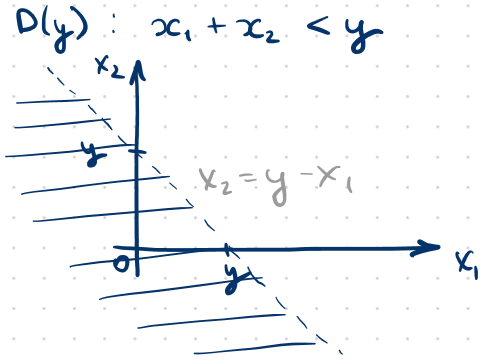
\includegraphics[width=\linewidth]{img/1.png}
\end{wrapfigure}  

Тогда $f_Y(y) = \int_{-\infty}^{+\infty} f_{X_1}(x_1)f_{X_2}(y-x_1) \, dx_1$ -- \textbf{функция свертки}.

\textbf{Доказательство}. $F_Y(y) = P\{Y<y\} = P\{X_1 + X_2 < y\} = \int \int_{D(y)} f(x_1, x_2) \, dx_1 \,dx_2 = \int_{-\infty}^{+\infty} \, dx_1 \int_{-\infty}^{y-x_1} f(x_1, x_2) \,dx_2 = \zigzagline x_1, x_2 \text{-- независимы}, f(x_1, x_2) = f_{X_1}(x_1)f_{X_2}(x_2) \zigzagline = \int_{-\infty}^{+\infty} \, dx_1 f_{X_1}(x_1) \int_{-\infty}^{y-x_1} f_{X_2}(x_2) \,dx_2 = \int_{-\infty}^{+\infty} \, dx_1 f_{X_1}(x_1) F_{X_2}(y-x_1)$. Продифференцируем: $f_Y(y) = \frac{d}{dy}(F_Y(y)) = [\int_{-\infty}^{+\infty} f_{X_1}(x_1) F_{X_2}(y-x_1) \, dx_1]' = \zigzagline \frac{d}{dy}(F_{X_2}(y-x_1)) = f_{X_2}(y-x_1) \zigzagline = \int_{-\infty}^{+\infty} f_{X_1}(x_1) f_{X_2}(y-x_1) \, dx_1$.

\section{Сформулировать определение математического ожидания случайной величины (дискретный и непрерывный случаи). Записать формулы для вычисления математического ожидания функции от случайной величины. Сформулировать свойства математического ожидания. Механический смысл математического ожидания}

\begin{wrapfigure}{l}{0.5\textwidth}
	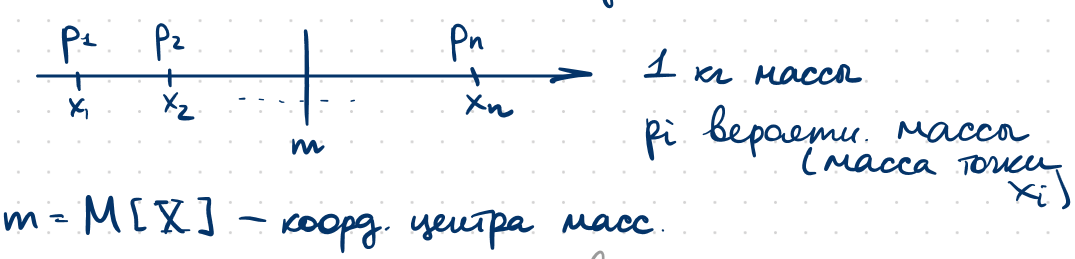
\includegraphics[width=\linewidth]{img/2.png}
\end{wrapfigure}  

Пусть $X$ -- \textbf{дискретная} случайная величина. \textbf{Математическое ожидание} (среднее значение) случайной величины $X: M[X] = \sum_{i} x_ip_i,$ где $p_i = P\{X=x_i\}$, $i$ пробегает все номера элементов конечного множества значений случайной величины.

\begin{wrapfigure}{r}{0.5\textwidth}
	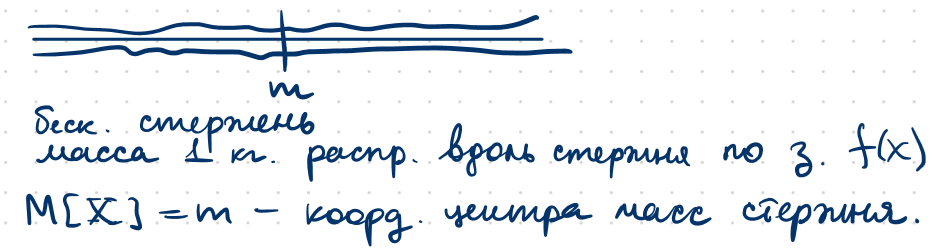
\includegraphics[width=\linewidth]{img/3.png}
\end{wrapfigure}  

Пусть $X$ -- \textbf{непрерывная} случайная величина, $f_X(x)$ -- плотность распределения. \textbf{Математическое ожидание} (среднее значение) случайной величины $X: M[X] = \int_{-\infty}^{+\infty} xf(x)\, dx$.


\textbf{Свойства}:
\begin{enumerate}
	\item $X$ -- случайная величина, $\varphi: \mathbb{R} \rightarrow \mathbb{R}$:
	\begin{itemize}
		\item $M[\varphi(X)] = \sum_{i} \varphi(x_i)p_i$, если $X$ -- дискретная случайная величина;
		\item}$M[\varphi(X)] = \int_{-\infty}^{+\infty} \varphi(x)f(x) \, dx$, если $X$ -- непрерывная случайная величина, $f(x)$ -- плотность;
	\end{itemize}
	\item $\vec{X} = (X_1, X_2)$ -- случайный вектор, $\varphi: \mathbb{R}^2 \rightarrow \mathbb{R}, Y = \varphi(X_1, X_2)$. $p_{ij} = P_i\{(X_1, X_2) = (x_{1, i}, x_{2, j})\}$:
	\begin{itemize}
		\item $M[\varphi(X_1, X_2)] = \sum_{i, j} \varphi (x_{1, i}, x_{2, j})p_{ij}$, если $\vec{X}$ -- дискретный вектор;
		\item $M[\varphi(X_1, X_2)] = \int_{-\infty}^{+\infty} \int_{-\infty}^{+\infty} \varphi(x_1, x_2)f(x_1, x_2) \, dx_1 \, dx_2$, где $f(x_1, x_2)$ -- совместная плотность непрерывного случайного вектора $\vec{X}$.
	\end{itemize}
\end{enumerate}

\section{Сформулировать определение дисперсии случайной величины. Записать формулы для вычисления дисперсии в дискретном и непрерывном случае. Сформулировать свойства дисперсии. Механический смысл дисперсии}

\textbf{Дисперсией} случайной величины $X$ называется $DX = M[(X-m)^2],$ где $m=MX$.

Если $X$ -- \textbf{дискретная} случайная величина, то $DX = \sum_{i} (x_i - m)^2 p_i$, где $p_i = P\{X=x_i\}$. Если  $X$ -- \textbf{непрерывная} случайная величина, то $DX = \int_{-\infty}^{+\infty} (x-m)^2f(x) \, dx$, где $f$ -- функция плотности случайной величины $X$.

\textbf{Свойства}:
\begin{enumerate}
	\item для любого случайного вектора $X: DX \geq 0$;
	\item если $P\{X=x_0\} = 1,$ то $DX = 0$;
	\item $D[aX+b] = a^2DX,      a, b = const$;
	\item $D[X] = M[X^2] - (MX)^2$;
	\item если $X_1, X_2$ -- независимые случайные величины, то $D[X_1 + X_2] = D[X_1] + D[X_2]$.
\end{enumerate}

\textbf{Механический смысл дисперсии:} дисперсия является моментом инерции вероятностной массы относительно точки $m=MX$, т.е. характеризует <<разброс>> вероятностной массы относительно математического ожидания этой случайной величины. Чем больше $D$, тем больше <<разброс>>.

\section{Сформулировать определения начального и центрального моментов случайной величины. Математическое ожидание и дисперсия как моменты. Сформулировать определение квантили и медианы случайной величины}

Пусть $X$ -- случайная величина. \textbf{Моментом} $k^{\text{ого}}$ порядка ($k$-м моментом, $k$-м \textbf{начальным} моментом) случайной величины $X$ называется число $mk = M[X^k]$.

Если $X$ -- дискретная случайная величина, то $m_k = \zigzagline M[\varphi(x)] = \sum_{i} \varphi(x_i)p_i \zigzagline = \sum_{i} x_i^kp_i$.

Если $X$ -- непрерывная случайная величина, то $m_k = \int_{-\infty}^{+\infty} x^kf(x) \, dx$.

\textbf{Центральным моментом} $k^{\text{ого}}$ порядка случайной величины $X$ называется число $m^\circ k = M[(X-MX)^k]$.

Если $X$ -- дискретная случайная величина, то $m_k^\circ =\sum_{i}(x_i-MX)^kp_i$.

Если $X$ -- непрерывная случайная величина, то $m_k^\circ = \int_{-\infty}^{+\infty} (x-MX)^k f(x) \, dx$.

$m_2^\circ = DX, m_1^\circ = 0.$

Математическое ожидание случайной величины $Х$ совпадает с моментом первого порядка. Дисперсия совпадает с центральным моментом 2-го порядка.

Пусть $X$ - случайная величина, $\alpha \in (0, 1)$. \textbf{Квантилью} уровня $\alpha$ случайной величины $X$ называют число $q_\alpha$, для которого: $P\{X < q_\alpha\} \leq \alpha, P\{X>q_\alpha\} \leq 1 - \alpha$.

\textbf{Медианой} случайной величины $X$ называется ее квантиль уровня $\frac{1}{2}$.

\section{Сформулировать определение ковариации случайных величин. Записать формулы для вычисления ковариации в дискретном и непрерывном случаях. Сформулировать свойства ковариации}

Ковариация является числовой характиристикой случайного вектора. Пусть $(X_1, X_2)$ -- двумерный случайный вектор. $Ковариацией$ случайной величины $X_1$ и $X_2$ называется число $cov(X_1, X_2) = M[(X_1 - m_1)(X_2 - m_2)],$ где $m_i = MX_i, i = \overline{1, 2}$.

Если $X_1, X_2$ - дискретный случайные величины, то $cov(X_1, X_2) = \sum_{i_1, i_2}(x_{1, i_1}-m_1)(x_{2, i_2}-m_2)p_{i_1i_2},$ где $p_{i_1i_2} = P\{(X_1, X_2) = (x_{1, i_1}, x_{2, i_2})\}$.

Если $X_1, X_2$ - непрерывные случайные величины, то $cov(X_1, X_2) = \int \int_{\mathbb{R}} (x_1 - m_1)(x_2 - m_2) f(x_1, x_2) \, dx_1 \,dx_2$, где $f$ -- совместная плотность распределения $X_1$ и $X_2$.

\textbf{Свойства}:
\begin{enumerate}
	\item $D[X+Y] = DX + DY + 2cov(X, Y)$;
	\item $cov(X, X) = DX$;
	\item если $X, Y$ -- независимы, то $cov(X, Y) = 0.$ Обратное не верно;
	\item $cov(a_1X + b_1, a_2Y + b_2) = a_1a_2cov(X, Y)$;
	\item $|cov(X, Y)| \leq \sqrt{DX \cdot DY}$, причем $|cov(X, Y)| = \sqrt{DX \cdot DY} \equiv$ случайные величины $X$ и $Y$ связаны линейной зависимостью;
	\item $cov(X, Y) = M[XY] - (MX)(MY)$.
\end{enumerate}